\documentclass[oneside,a4paper,12pt,headsepline,cleardoubleempty,%
    pointlessnumbers,bibtotoc]{scrreprt}
    
\usepackage{APackages}

\usepackage{inputenc}	% erlaubt von US-ASCII verschiedene Zeichenkodierung
\inputencoding{utf8}		% Wir wollen UTF-8 (=keine Probleme mit Umlauten etc.)

\pagestyle{plain}	% leere Seitenstil (keine Seitennummern usw.)
%\numberwithin{equation}{subsection}
%\renewcommand{\theequation}{\arabic{section}.\arabic{subsection}.\arabic{equation}}
%\numberwithin{figure}{section}
%\renewcommand{\thefigure}{\arabic{section}.\arabic{figure}}

% add text color
\usepackage{color}

% technical name definitions
\newcommand{\amiro}{AMiRo}
\newcommand{\amiros}{AMiRos}
\newcommand{\diwheel}{{\it DiWheelDrive}}
\newcommand{\power}{{\it PowerBoard}}
\newcommand{\proxring}{{\it ProximityRing}}
\newcommand{\light}{{\it LightRing}}
\newcommand{\cognition}{{\it CognitionBoard}}
\newcommand{\imageproc}{{\it ImageProcessing}}
\newcommand{\progcable}{{\it programming cable}}

% paths and program names
\newcommand{\muroxdocu}{\textcolor{blue}{\url{www.multirobotix.de/dokuwiki/doku.php}}}
\newcommand{\rsbdocu}{\textcolor{blue}{\url{docs.cor-lab.de}}}
\newcommand{\utilitypath}{{\tt project/utilities/}}
\newcommand{\utilitypathI}{{\it project/utilities/}}
\newcommand{\demopath}{{\tt project/demo/}}
\newcommand{\demopathI}{{\it project/demo/}}
\newcommand{\amirohomepath}{{\tt root/}}
\newcommand{\amirohomepathI}{{\it root/}}
\newcommand{\testname}{{\tt braitenberg}}
\newcommand{\testnameI}{{\it braitenberg}}
\newcommand{\initialname}{{\tt initial}}
\newcommand{\initialnameI}{{\it initial}}
\newcommand{\stoppath}{{\tt project/tools/robotTools/}}
\newcommand{\stoppathI}{{\it project/tools/robotTools/}}
\newcommand{\stopname}{{\tt stopAMiRo}}
\newcommand{\stopnameI}{{\it stopAMiRo}}
\newcommand{\setlightspath}{{\tt project/act/}}
\newcommand{\setlightspathI}{{\it project/act/}}
\newcommand{\setlightsname}{{\tt setLights}}
\newcommand{\setlightsnameI}{{\it setLights}}

% module and additional program names
\newcommand{\modulemurox}{{\tt murox/env}}
\newcommand{\gtk}{GTKTerm}
\newcommand{\gtkC}{gtkterm}

% other markings
\newcommand{\noref}{\textcolor{red}{???}}
\newcommand{\working}{\textcolor{red}{\bf $>>>$ topic in progress $<<<$}}


\hyphenation{}

% Ende der Voreinstellungen

\begin{document}
\pagenumbering{roman}

\title{\amiro\ Cheatsheet \\ }
%\subtitle{\includegraphics[scale=0.1]{Bilder/AMiRos02.JPG}}
\subtitle{\includegraphics[scale=0.3]{Bilder/AMiRos03.png}}
\date{Last Update: September 2016}

\maketitle



\newpage

\tableofcontents

%\listoffigures

\newpage
\pagenumbering{arabic}

\chapter{What is the \amiro ?}

The \amiro\ - {\bf A}utonomous {\bf Mi}ni {\bf Ro}bot - is a mini robot for research and education. Basic algorithms can be implemented and evaluated very easily due to small requirements. The construction is modular, where each module has its own processing unit. The modules are connected by a CAN bus. The basic modules are the \diwheel, the \power\ and the \light\ as shown in figure \ref{fig:allModules}(a, b, d) and in figure \ref{fig:stackedModules}.

\begin{figure}[htb]
\begin{center}
\begin{tabular}{ccc}
\includegraphics[scale=1.5]{Bilder/boardpics/lightring.png} &
\includegraphics[scale=1.5]{Bilder/boardpics/diwheeldrive.png} &
\includegraphics[scale=1.5]{Bilder/boardpics/cognitionboard.png} \\
(a) \light & (b) \diwheel & (c) \cognition \\
\includegraphics[scale=1.5]{Bilder/boardpics/powerboard.png} &
\includegraphics[scale=1.5]{Bilder/boardpics/proxring.png} &
\includegraphics[scale=1.5]{Bilder/boardpics/imageproc.png} \\
(d) \power & (e) \proxring & (f) \imageproc \\
\end{tabular}
\caption{Current set of \amiro\ modules.}
\label{fig:allModules}
\end{center}
\end{figure}

The \diwheel\ (figure \ref{fig:allModules}(b)) is for drive control, position estimation and ground detection. By using a STMicroelectronics ARM Cortex-M3 based STM32F103 MCU, it controls the motors by receiving driving commands and calculating the rotation speed for the odometry. It also gives the position of the robot by magnetometer, accelerometer and gyroscope. Additionally by using proximity sensors at the bottom, it can detect the ground.

The \power\ (figure \ref{fig:allModules}(d)) is basically responsible for the power supply. It has the battery fuel gauge and charger and the voltage regulators for different voltage connections. Additionally it controls the \proxring\ around the \amiro\ (figure \ref{fig:allModules}(e)), which contains eight infrared proximity sensors and four capacity touch sensors, and the wireless communication via bluetooth. For the processes a STMicroelectronics ARM Cortex-M4 based STM32F104 MCU is used, which also consists of a FPU.

The \light\ (figure \ref{fig:allModules}(a)) is for status visualization and optical communication. Additionally sensor extensions like a laser scanner, which is not included in the \amiro, can be connected. The processing unit is the same MCU as on the \diwheel.

\begin{figure}[htb]
\begin{center}
\begin{tabular}{ccc}
\includegraphics[scale=0.4]{Bilder/amiroDiWheel.png} &
\includegraphics[scale=0.4]{Bilder/amiroPower.png} &
\includegraphics[scale=0.4]{Bilder/amiroLight.png} \\
(a) \diwheel & (b) \power & (c) \light \\
\end{tabular}
\caption{Front view of the modules of the \amiro. Between the \power\ and the \light\ there can be stacked module extensions like the \cognition.}
\label{fig:stackedModules}
\end{center}
\end{figure}

%\begin{figure}[htb]
%\begin{center}
%\includegraphics[scale=1.2]{Bilder/schematic_side.png}
%\caption{Schematic of the front view of the \amiro\ and its modules.}
%\label{fig:schematicModules}
%\end{center}
%\end{figure}

Between the \power\ and the \light\ there can be stacked module extensions as shown in figure \ref{fig:stackedModules}. The most interesting module for this cheatsheet is the \cognition\ (figure \ref{fig:allModules}(c)). It contains a Gumstix Overo TidalSTORM COM, which combines an ARM Cortex-A8 based DaVinci DM3730 SoC from Texas Instruments running at \unit[1]{GHz} with \unit[1]{GB} RAM and a micro SD card as hard drive. An usual Linux operating system is installed. By using the CAN bus the sensor data from the other modules can be loaded and commands can be sent. Additionally it has an own wireless communication card and an additional micro USB slot, so the \cognition\ can be connected to any wired or wireless IP connection.

Additionally the \imageproc\ (figure \ref{fig:allModules}(f)) could be added, which isn't finally developed yet. It shall contain a FPGA for parallel image processing.

On the title page different \amiros\ are shown. The left \amiro\ in the foreground, which is touched by a hand, is the basic \amiro\ only consisting the modules \diwheel, \power\ and \light\ with its lights turned on. The right \amiro\ in the foreground (its front is to the left side) doesn't have its chasis and its \proxring. The wheels at its sides and the battery packs in its front and back can be seen. Additionally it consists of the extension modules \cognition\ and \imageproc\ between the \power\ and the \light, so it is higher than the left \amiro. At its front, the small camera, which is connected to the \cognition, can be seen. In the background there are several \amiros\ with different sensor extensions like a laser scanner or a RGBD camera (camera with pixel values consisting of {\bf r}ed, {\bf g}reen and {\bf b}lue channels and {\bf d}epth) on top of the robots.

%On the title page two different \amiros\ are shown. On the right side there is the basic \amiro\ only consisting the modules \diwheel, \power\ and \light\ with its lights turned on. On the left side there is an extended \amiro. It also contains the \cognition, wherefore it is higher, and a laser scanner has been placed on top of it. Finally the internal camera has been installed, so the \amiro\ has got an additional circular cutting in the front.

In the following chapters the descriptions and algorithms are designed for the \cognition. The basic modules \diwheel, \power\ and \light\ will only be used, but not programmed or changed.

\chapter{What do we need at first?}

For basic communication between the computer and the \amiro, the \progcable\ which is shown in figure \ref{fig:cables}(a) is needed. It can be used for basic console commands on all boards and for flashing new programms on the microcontrollers of the \diwheel, \power\ and the \light.

\begin{figure}[htb]
\begin{center}
\begin{tabular}{cc}
\includegraphics[scale=0.05]{Bilder/ProgCable.JPG} &
\includegraphics[scale=0.05]{Bilder/USBCable.JPG} \\
(a) & (b) \\
\end{tabular}
\caption{The \progcable\ (a) and micro USB cable (b).}
\label{fig:cables}
\end{center}
\end{figure}

For copying programs on the \cognition\ a ssh connection is needed. This can be accomplished in different ways:
\begin{itemize}
\item Using a {\it micro USB cable}:

The {\it micro USB cable}, which is shown in figure \ref{fig:cables}(b), has to be pluged into the micro USB connector of the \cognition. The basic IP address for the ssh connection for every \amiro\ is 192.168.3.1. On Linux machines there has to be initialized an {\it usb0 interface} with the IP address 192.168.3.$<$2-255$>$.

\item Using the {\it citopenrobotix} network:

With the internal network card on the \cognition\ the \amiros\ connect themselfs to the {\it citopenrobotix} network automatically. The computer just has to be in the same network. By typing {\it ifconfig} into the console of the \cognition\ the IP address of the \amiro\ can be read.
\end{itemize}

\section{Access to murox Repository}

The programs for the Linux evironment of the \cognition\ are stored in the murox repository. Please contact the supervisor for the link and the access data. The murox repository is a git repository, which has to be cloned recursively on the computer. The structure is described in chapter \ref{sec:structuremurox}. The programs have to be copied on the \cognition\ via a ssh connection.

To build the projects of the murox repository, it has to be initialized:
\begin{enumerate}
\item Open the console on the computer.
\item Go to the cloned murox repository.
\item Got to the {\it usability} folder: {\tt\$ cd \utilitypath}
\item Execute initialization script: {\tt\$ ./initMurox}
\item Go to home directory: {\tt\$ cd}
\item Source the bashrc: {\tt\$ source .bashrc}
\end{enumerate}
Now global variables for murox path specifications have been added to the bashrc. Do not change the additions manually. If the murox repository has been moved, the paths have to be reinitialized. In this case the murox lines in the bashrc just have to be removed and the described initialization has to be done again.

\section{Initialization of \gtk}

\gtk\ is a program for serial communication. It is needed to have access to the consoles of the \amiro\ boards. For the connection with the \amiro, the configuration file of \gtk\ has to be edited:
\begin{enumerate}
\item Open the configuration file: {\tt\$ nano \textasciitilde/.gtktermrc}
\item Change the following lines as shown:\\
{\tt > port = /dev/ttyUSB0} \\
{\tt > speed = 115200} \\
{\tt > crlfauto = True}
\end{enumerate}

\section{Start and Connect the \amiro}

For starting and connecting with the \amiro\ there is a basic procedure:
\begin{enumerate}
\item Plug the \progcable\ into the computer.
\item Start \gtk: {\tt\$ \gtkC}
\item Reset RTS flag by pressing F8 (the RTS flag in the right bottom corner has to be gray).
\item Plug the \progcable\ into the serial slot of the \diwheel.
\end{enumerate}
If the \amiro\ is shutdowned, the RTS flag has to be set and reset by double pressing F8 again.

The RTS flag is the reset flag for the \amiro. If it is set, all processing units on the boards are turned off. If the flag is reset, all processing units are running. \gtk\ automatically sets the RTS flag. If the \amiro\ is turned on and the \progcable\ is beeing pluged in, the \amiro\ will be turned off without any save shutdown procedure. This is the reason, why the flag has to be reset befor pluging in the \progcable.

After the described procedure the \amiro\ turns on and in the console output of \gtk\ there should be running an interactive console. By for example typing {\it help} a list of all console commands of the \diwheel\ will be shown. For getting access on the console of the \cognition, the following steps have to be done:

\begin{enumerate}
\item Unplug the \progcable\ from the \diwheel\ only.
\item Plug the \progcable\ into the serial slot of the \cognition.
\end{enumerate}

If this is done directly after turning the \amiro\ on, there will be the setup output of the Linux operating system. Soon the login request will be shown. If there is no console output showing by \gtk, please press return. The login request should be shown now.

If the supervisor doesn't give any login information, the basic login is {\it root}. If it is asked for a password, just press return. Now basic Linux commands can be used for navigation and execution like in any other Linux console.

\section{Stopping and Shutting down the \amiro}
\label{sec:stopshutdown}

If a program of the \cognition\ is broken or has been stopped, all functions, which are controlled by this program, will be stopped on the \cognition. But there are also functionalities, which are not controlled by any program of the \cognition\ like the motor control, which is done by the \diwheel. If a program for example sets motor speeds and breaks, the motors will continue driving.

For really stopping the \amiro, it is important to execute the stop tool \stopnameI\ in \stoppathI\ on the \cognition. It stops the motors and resets the lights to the initial colors of the \light.

For shutting down the \amiro, please do the following steps:
\begin{enumerate}
\item Plug the \progcable\ into the \diwheel\ (the RTS flag has to be reset!)
\item Type the shutdown command for deep sleep: {\tt\$ shutdown d}
\end{enumerate}
The \progcable\ can be unplugged now. The \amiro\ starts the save shutdown procedure. Please, do not use the RTS flag for shutting down. If the flag is set, the \amiro\ is turned off, but when the \progcable\ will be unplugged, the \amiro\ restarts.

\section{Building and Running first Program}
\label{sec:firstprog}

At first the program has to be build. Please follow the following steps:

\begin{enumerate}
\item Open the console on the computer.
\item Go to the cloned murox repository.
\item Go to the project: {\tt\$ cd \demopath\testname}
\item Load the murox environment: {\tt\$ module load \modulemurox}
\item Build the project: {\tt\$ ./build.sh}
\end{enumerate}

Now the project is build for the \amiro. For copying and starting the program example the ssh connection to the \amiro\ is needed:

\begin{enumerate}
\item Copy the project on the \amiro: {\tt\$ ./copyprograms <\amiro\ IP address>}
\item Open console of the \cognition\ of the \amiro.
\item Go to the project: {\tt\$ cd \amirohomepath\testname}
\item Start program: {\tt\$ ./runSimple.sh}
\end{enumerate}

Now the \amiro\ behaves like a very simple Braitenberg vehicle. It drives forward and turns if there is an object by using the sensors of the \proxring. It doesn't stop in front of edges! To change the sensitivity open the script {\it runSimple.sh} and change the integer value of the parameter {\it -f}. The behavior of the proximity sensors in the \proxring\ is described in chapter \ref{sec:proxsensors}.

For stopping the program press strg+C and execute {\it stop.sh} afterwards. The execution of the stop tool \stopnameI, which has been described in chapter \ref{sec:stopshutdown}, is already included in the stop script, so it doesn't have to be executed manually.

\chapter{\amiro's Setup}
\label{sec:amirosetup}

Some sensors of the \amiro\ need a setup before they can be used efficiently. For sensor details please have a look into chapter \ref{sec:sensors}. For the sensor initialization there is a project, which has to be build and copied on the \amiro\ (by using ssh connection):

\begin{enumerate}
\item Open the console on the computer.
\item Go to the cloned murox repository.
\item Go to the initial project: {\tt\$ cd \demopath\initialname}
\item Load the murox environment: {\tt\$ module load \modulemurox}
\item Build the project: {\tt\$ ./build.sh}
\item Copy the project: {\tt\$ ./copyPrograms.sh <\amiro\ IP address>}
\item Open the console on the \cognition\ of the \amiro.
\item Go to the initial project: {\tt\$ cd \amirohomepath\initialname}
\end{enumerate}

Now there are different scripts for the initialization of the sensors. Please have a look into chapter \ref{sec:sensors} for the initialization details of the needed sensor.

\section{Program Example with Setup}
\label{sec:firstprogsetup}

At first execute the initialization of the \proxring, which is described in chapter \ref{sec:proxsensors}. Afterwards just build and copy the Braitenberg program as described in chapter \ref{sec:firstprog}.

Before execution, please check, if in \amirohomepathI\initialnameI\ there exist the files {\it irConfig.conf} and {\it irEmpty.conf} and if the ground offsets belong to the ground the \amiro\ shall now drive on. Then execute the script {\it runStandard.sh}.

The \amiro\ behaves like a simple Braitenberg vehicle again, but now it is more sensitive to objects and it can detect table edges. Due to the initialization of the \proxring, an obstacle and an edge model can be used for precise distance calculations.


\chapter{Structure of murox Repository}
\label{sec:structuremurox}

The murox repository contains several programs for the \cognition. These are sorted into different subdirectories based on their functionality. All programs and the structure is documented in the murox documentation: \\
\muroxdocu \\
Please contact your supervisor for login information.

Basically there are seven subdirectories:

\medskip

\begin{tabular}{c|l}
{\bf Subdirectory} & {\bf Description} \\
\hline
demo & Demos of the \amiro. A demo is a conclusion of programs, which are \\
     & implemented in the other directories. In demos there are only scripts \\
     & and executables, but there isn't any program code. \\
\hline
sense & All sensing tools (sensors, cameras, etc.). \\
\hline
act & All tools for executing actions (motors, lights). \\
\hline
process & All processing tools including exploration, navigation, object \\
        & detection, statemachines, etc. \\
\hline
tools & Tools for testing or stopping procedures on the \amiro\ or tools for \\
      & communication between the computer and the \amiro.\\
\hline
sandbox & Development directory. All programs and demos, which are still in \\
        & development and are not runnable or functional, are stored here. \\
\hline
includes & All programs and headers, which are included in the other programs, \\
         & for example headers for \amiro\ and CAN constants. \\
\end{tabular}

\bigskip

For the \amiro\ there can be implemented {\bf programs} and there can be designed {\bf demos}. A program contains program code and can be built directly. A demo concludes some programs to one project, but there isn't any program code. In a demo the referenced programs can be built and only their executables are stored in this project. Additionally there can be added some scripts for faster executions and communications.

If a new project shall be created with new programs, the new demo and the new programs will be stored in {\it sandbox} at first. Here are stored all not runnable or functional programs and demos. Later, if it's running stable, the program will be moved to one of the directories {\it sense}, {\it act}, {\it process} or {\it tools} based on its functionality. A stable demo will be moved to the directory {\it demo}.

\section{Robotic Service Bus (RSB)}

The {\bf R}obitic {\bf S}ervice {\bf B}us (RSB) is a message-oriented, event-driven middleware. It is the basic communication framework for all murox programs, which are cooperating with each other. For example the sense tools, which are described in chapter \ref{sec:sensetools}, are publishing their sensor data via RSB. For a full documentation of RSB and for program examples in different programming languages, please visit the Cor-Lab's documentation website: \\
\rsbdocu

If many programs are publishing and receiving data via RSB, it is very important to get an overview about the published scopes by the RSB logger. The following commands are possible:

\medskip

\begin{tabular}{l|l}
{\bf RSB logger command} & {\bf Description} \\
\hline
{\tt rsb-loggercpp0.11} & Gives an overview about all scopes and their \\
\quad {\tt -{}-style monitor <scope>} & publication frequency, which are under the given \\
& scope. \\
\hline
{\tt rsb-loggercpp0.11} & Gives all details about the published packages \\
\quad {\tt -{}-style detailed <scope>} & of all scopes, which are under the given scope. \\
\end{tabular}

\bigskip

The Braitenberg demo, which has been presented in the chapters \ref{sec:firstprog} and \ref{sec:firstprogsetup}, consists of two basic programs: the main Braitenberg behavior calculation in {\it braitenberg} and the reading of the proximity sensors of the \proxring\ by {\it senseRingProximity}. The last tool publishs the read sensor data via RSB, which can be received by the main program. In the following subsections the RSB logger output for both demos will be presented.

\subsection{RSB Logger of Simple Braitenberg Demo}

If the simple Braitenberg demo will be started like in chapter \ref{sec:firstprog}, an RSB communication overview can be called by the following command: \\
{\tt\$ rsb-loggercpp0.11 -{}-style monitor /}

\begin{figure}[htb]
\begin{center}
\includegraphics[scale=0.6]{Bilder/rsbloggerpics/rsb_br_simple_monitor.png}
\caption{Monitor style output of the RSB logger of the simple Braitenberg demo.}
\label{fig:rsbloggersimplemonitor}
\end{center}
\end{figure}

As shown in figure \ref{fig:rsbloggersimplemonitor} all RSB communication scopes are printed, which start with "/". For every scope the latency in micro seconds and the frequency is listed.

If there are needed more detailed information about for example the sensor data publications,  the RSB logger can be called as follows: \\
{\tt\$ rsb-loggercpp0.11 -{}-style detailed /rir\_prox/original} \\
Now the RSB logger gives every detailed information about every package that is published via the given scope. This example is shown in figure \ref{fig:rsbloggersimpledetailed}. The most important information is the scope name, the type and the payload. In this case it is a byte array of 36 bytes. The values themselves are hard to read, but in this case relative value changes can be checked.

\subsection{RSB Logger of Standard Braitenberg Demo}

The standard version of the braitenberg demo, which has been built and started in chapter \ref{sec:firstprogsetup}, can also be analized like the simple version in the foreign chapter: \\
{\tt\$ rsb-loggercpp0.11 -{}-style monitor /}

\begin{figure}[htb]
\begin{center}
\includegraphics[scale=0.6]{Bilder/rsbloggerpics/rsb_br_standard_monitor.png}
\caption{Monitor style output of the RSB logger of the standard Braitenberg demo.}
\label{fig:rsbloggerstandardmonitor}
\end{center}
\end{figure}

But this time the scope list of the RSB logger, which is shown in figure \ref{fig:rsbloggerstandardmonitor}, is longer. The {\it senseRingProximity} tool doesn't send the original proximity sensor values only, but the sensor values for the obstacle and the ground model, too. This is the reason for the three subscopes for {\it /rir\_prox}. Additionally there is a scope, which is used by the main program itself. It publishs commands.

For getting more information about the RSB packages of the {\it senseRingProximity} tool, the main scope can be choosen: \\
{\tt\$ rsb-loggercpp0.11 -{}-style detailed /rir\_prox} \\
Now all packages of the three subscopes are shown. For getting information about just the packages of only one scope, the full scope name can be used: \\
{\tt\$ rsb-loggercpp0.11 -{}-style detailed /rir\_prox/obstacle} \\
As shown in figure \ref{fig:rsbloggerstandarddetailed}(a) and \ref{fig:rsbloggersimpledetailed}, the packages sent by {\it senseRingProximity} have all the same structure.

For getting more information about te command packages of the main program, the following command has to be typed: \\
{\tt\$ rsb-loggercpp0.11 -{}-style detailed /frontObject/command} \\
The type of the package, which is shown in figure \ref{fig:rsbloggerstandarddetailed}(b), is a standard string and the payload consists of 4 readable chars: STOP. This is the command, which is sent, when the robot is in front of an object. It can be received and used by for example an object detection, which shall only detect objects, if there is something in front of the robot. Behaviors like this can for example save energy.


\section{Useful Sense and Act Tools}
\label{sec:sensetools}

For the most sensors there already exist sense tools, which read the sensors' values and publish them via RSB:
\begin{itemize}
\item {\bf sendOdometry<publish type>:} \\
Reads the odometry from the \diwheel\ and publishs the values via RSB based on the RSB type included in the tool name.

\item {\bf senseCam<publish type>:} \\
Catchs the images of the internal camera. The image will be compressed and published via RSB based on the RSB type included in the tool name.

\item {\bf senseFloorProximity:} \\
Reads the floor proximity sensors, which are at the bottom of the \amiro. The values are published via RSB as an integer vector (see chapter \ref{sec:proxsensors}).

\item {\bf senseHokuyo:} \\
Reads the values of the Hokuyo Laser Scanner. The published RSB type is\\
{\tt rst::vision::LocatedLaserScan}.\\
This type includes the laser scans and all parameters of the laser scanner like laser count, angular ranges, etc. Basically this sense tool can be used for different laser scanners with different laser scan parameters. For now it is specialized in the Hokuyo Laser Scanner.

\item {\bf senseRingProximity:} \\
Reads the proximity sensors of the \proxring. The values are published in three different variants via RSB as an integer vector: As original values, values for the obstacle model and as values for the edge model. For the models the configuration files {\it irConfig.conf} and {\it irEmpty.conf} are loaded from the directory \amirohomepathI\initialnameI. While the air offsets can only be read at the beginning, the ground offsets can be changed at runtime by giving a path to another ground offset file. For more detailed information about the offsets, please have a look into chapter \ref{sec:proxsensors}.

\item {\bf setLights:} \\
This tool sets the lights to given colors. Additionally it cannot let the LEDs only shine, but it can let them blink in different ways in a given period time. Please have a look into chapter \ref{sec:lights} for more detailed information.
\end{itemize}

\section{Useful Runnable Demos}
% IMPORTANT: Here are only demos, which can be run without any robot extension like a laser scanner!

The following demos in the directory \demopathI\ can be build and run on the \amiro\ easily.

\subsection{initial}

This demo is the most important one. It contains all setup scripts for sensor initializations and setup tests. For detailed information about the sensor initializations, please have a look into chapter \ref{sec:sensors}. The generated configuration files will be stored in this project. Finally any other project, which needs the configuration information, has access to this directory.

\subsection{braitenberg}

This demo already has been presented in the chapters \ref{sec:firstprog} and \ref{sec:firstprogsetup}. The \amiro\ behaves like a simple Braitenberg vehicle by only using the proximity sensors of the \proxring. There are three different variants the braitenberg demo can be started:
\begin{itemize}
\item {\bf simple:} By executing the script {\it runSimple.sh} the \amiro\ drives forward and turns in front of objects only by comparing the measurements with a simple threshold. There isn't any initialization needed.
\item {\bf standard:} By executing the script {\it runStandard.sh} the \amiro\ drives forward and turns in front of objects and table edges. For this behavior the initialization of the \proxring\ is needed, which is described in chapter \ref{sec:proxsensors}.
\item {\bf detect objects:} By executing the script {\it runObstacleStop.sh} the \amiro\ drives forward and turns in front of table edges. But this time it just stops in front of objects. By using the camera the \amiro\ sends an image via RSB, where the object is marked. Only if the object is taken the \amiro\ continues driving. Due to the obstacle and edge model based on proximity sensors, the \proxring\ has to be initialized (chapter \ref{sec:proxsensors}).
\end{itemize}

\subsection{follow\_ProximitySensors}

In this demo the \amiro\ follows an object, another \amiro\ or something else, which is in front of it, by only using the proximity sensors of the \proxring. The distances are calculated by the obstacle model of the proximity sensors, wherefore the \proxring\ has to be initialized, which is described in chapter \ref{sec:proxsensors}.

By executing the script {\it run.sh} all programs for the following behavior will be started, but the \amiro\ won't start following yet. By executing the script {\it follow.sh} the following command will be sent via RSB and the \amiro\ starts following the object, which is in front of it. By executing the script {\it wait.sh} the \amiro\ stops following due to the given stop command via RSB. The following and stop commands can be repeated. Finally for stopping the program, the script {\it stop.sh} has to be executed.

\chapter{Sense and Act with the \amiro}

The basic structure of the \amiro\ consisting of \diwheel, \power\ and \light\ contains many sensors and some actors. By using the \cognition\ the internal camera can also be used. Of course, there can be added external sensor and actor systems, but in this chapter only sensor and actor systems included in the \amiro\ will be presented.

\section{Sensors}
\label{sec:sensors}

The \amiro\ is a small sensor platform. While driving, the \diwheel\ calculates the movement by measuring the motor rotation speed with motor encoders. The \diwheel\ also contains gyroscope, accelerometer and magnetometer. The information of these sensors ca be used for example for odometry and position calculation.

For measuring the close environment there are used infrared proximity sensors. Four proximity sensors are at the bottom of the \amiro\ for ground detection (e.g. line detection), which are controlled by the \diwheel, and eight proximity sensors, which are controlled by the \power, are placed circular at the side of the chasis in the \proxring\ for a \unit[360]{$^{\circ}$} view around the robot.

The \proxring\ also includes four capacity touch sensors, two on each side. They can be used for human interaction very easily. The capacity touch sensors are also controlled by the \power.

Finally there is an included camera. It can only be controlled by the \cognition\ directly, so the basic \amiro\ structure, which only consists of \diwheel, \power\ and \light, doesn't contain the camera.

In the following subsections the sensors will be explained briefly. Additionally the usage for the Linux operating system on the \cognition\ will be described, including initialization information. The \cognition\ gets the sensor information of the other modules via the CAN bus.

\subsection{Odometry}

The odometry is only based on the motor encoders yet. An integration of gyroscope, accelerometer and magnetometer is still in development. The odometry can be set and read by the \cognition\ via the CAN bus. But there isn't any access to the encoders. The odometry will always be actualized by the \diwheel.

Additionally for odometry correction there can be set the kinematic calibration constants E$_{\text{d}}$ and E$_{\text{b}}$ based on the calibration by Jung and Chung \cite{JungChung}, which correct variation in wheel distance and wheel size proportion. These constants can be different for each \amiro.

For reading the odometry the sense tool {\it sendOdomtry} should be used. The usage and variants are described in chapter \ref{sec:sensetools}.

The CAN commands are:

\medskip

\begin{tabular}{l|l}
{\bf CAN command} & {\bf Description} \\
\hline
{\tt types::position getOdometry} & Gives the odometry as a TWB position type. \\
\hline
{\tt void setOdometry} & Sets the odometry to the given position \\
\quad {\tt types::position robotPosition} & {\it robotPosition}. \\
\hline
{\tt void setKinematicConstants} & Sets the kinematic calibration constants E$_{\text{d}}$ \\
\quad {\tt float Ed} & and E$_{\text{b}}$. \\
\quad {\tt float Eb} & \\
\end{tabular}

\subsection{Proximity Sensors}
\label{sec:proxsensors}

The proximity sensors at the bottom of the \amiro\ and in the \proxring\ are VCNL4020 infrared proximity sensors from Vishay. As shown in figure \ref{fig:proxis} the sensor consists of an infrared LED and the suitable infrared emitter for proximity calculations and additionally an ambient light emitter.

\begin{figure}[htb]
\begin{center}
\begin{tabular}{cc}
\includegraphics[scale=0.2]{Bilder/VCNL4020-Sensor.png} &
\includegraphics[scale=0.2]{Bilder/VCNL4020-Schematic.png} \\
(a) & (b) \\
\end{tabular}
\caption{The VCNL4020 sensor from Vishay (a) and its schematic (b).}
\label{fig:proxis}
\end{center}
\end{figure}

The ambient functionality isn't implemented yet. The sensors are only used for proximity calculations based on the measured infrared light reflections in the environment. Due to an internal integration of measurements while the infrared LED is turned on and off, the measured proximity value is nearly independed on the changing infrared light of the environment.

By using the floor proximity sensors at the \amiro's bottom, there can be done a ground detection. By using the proximity sensors of the \proxring, an obstacle avoidance can be implemented. For reading the proximity values the sense tools {\it senseFloorProximity} and {\it senseRingProximity} should be used only (see chapter \ref{sec:sensetools}). These tools give vectors with integer values. The ID assignment of the proximity sensors at the bottom of the \diwheel\ and in the \proxring\ is defined in figure \ref{fig:proxids}.

\begin{figure}[htb]
\begin{center}
\begin{tabular}{cc}
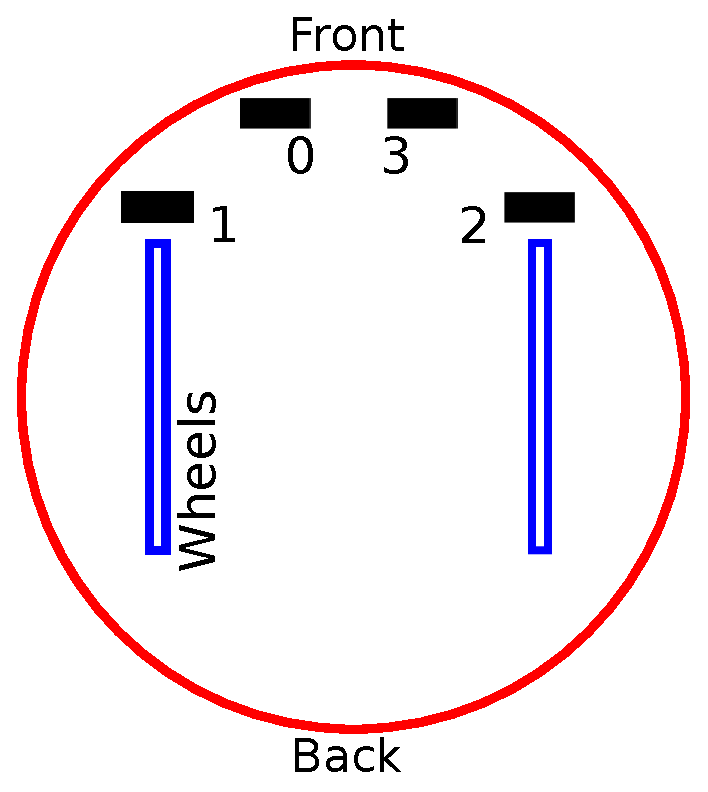
\includegraphics[scale=0.35]{Bilder/ProxFloorIDs.eps} &
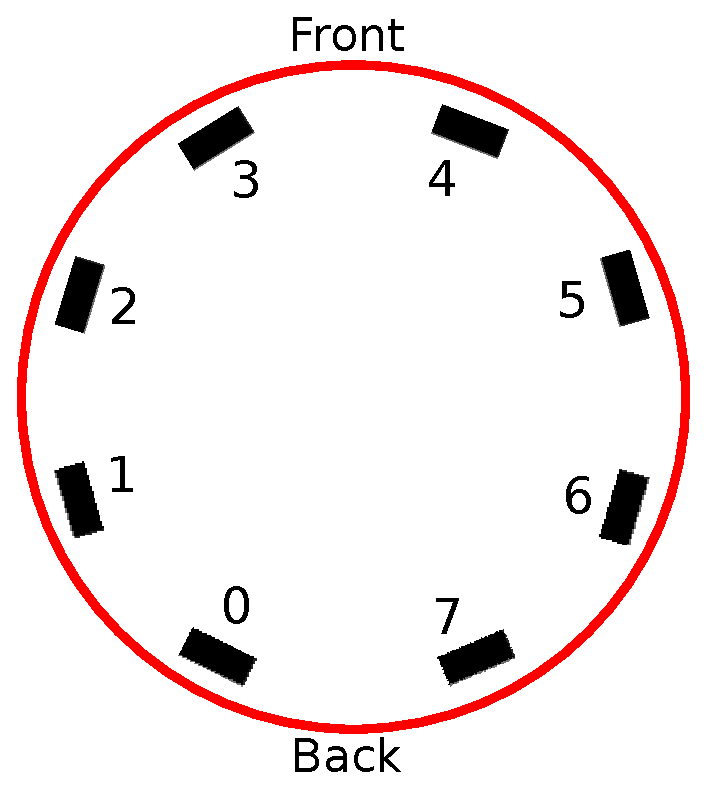
\includegraphics[scale=0.35]{Bilder/ProxRingIDs.eps} \\
(a) Bottom view of & (b) Top view of \\
\diwheel & \proxring \\
\end{tabular}
\caption{ID assignments of the proximity sensors on the \diwheel\ (a) and on the \proxring\ (b).}
\label{fig:proxids}
\end{center}
\end{figure}

\subsubsection{Interpretation of a Proximity Value}

A proximity value doesn't give any precise information about the environment. The reflection of the infrared light depends on the object's surface and color and, of course, on the objects count. One close object can effect the same proximity value than two objects of the same type farer away.

Additionally the position of one object isn't precise, either. An object, which is directly in front of the sensor, effects the same proximity value than an closer object of the same type at the side of the sensor. This is defined as the sensor's cone, which is shown in figure \ref{fig:proxcone}.

\begin{figure}[htb]
\begin{center}
\includegraphics[scale=0.3]{Bilder/VCNL4020-Cone.png}
\caption{The sensor's cone of the VCNL4020 sensor. Given a proximity value, an object (with known characteristics) can be anywhere on this cone.}
\label{fig:proxcone}
\end{center}
\end{figure}

In the subdirectory {\it includes} of the murox repository there is a sensor model for the VCNL4020 proximity sensors based on the proximity sensor model of Benet et. al. \cite{Benet_etal}. It can calculate the distance of an object by known angle and calculate the distance of a table edge. But this model needs an initialization of the proximity sensors, because the sensors' offsets are different.

\subsubsection{Initialization of the ProximityRing}

The \proxring\ has to be initialized. There are two offsets, which have to be measured for each sensor: The air offset (infrared light in the air) and the ground offset (infrared light reflected by the ground the robot stands on). Please build and copy the project \demopathI\initialnameI\ for the initialization (see chapter \ref{sec:amirosetup}). The needed scripts are stored in this project.

For the air offset the robot has to be placed without anything in its range (about \unit[25]{cm}). As shown in figure \ref{fig:proxinit}(a) the \amiro\ can be placed on a tall object, which has a hight of about \unit[25]{cm}. Now {\it runIREmpty.sh} has to be executed. This will take several minutes. Afterwards in the project folder there should be a file named {\it irEmpty.conf}, which contains the air offsets. This initialization has only to be done once per robot. Ideally the air offsets never change.

\begin{figure}[htb]
\begin{center}
\begin{tabular}{cc}
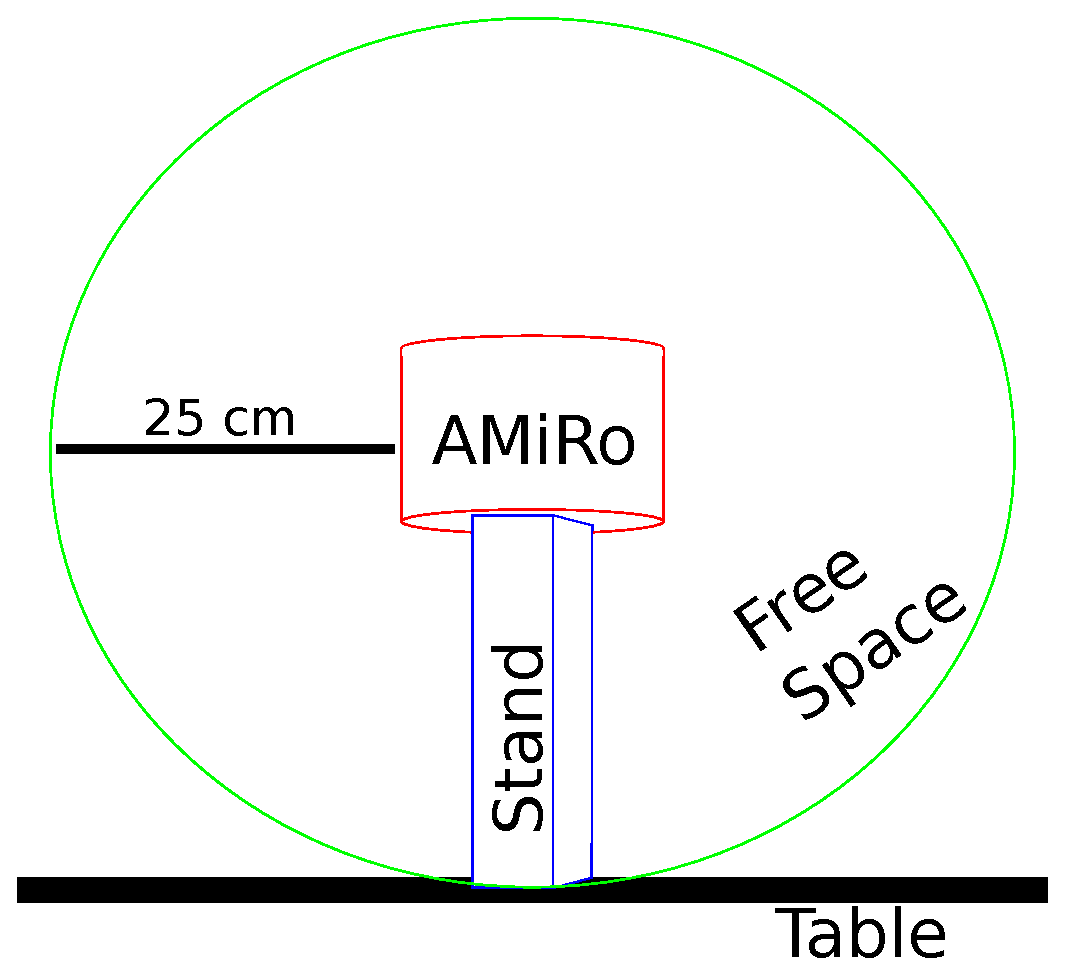
\includegraphics[scale=0.35]{Bilder/MeasAirOffset.eps} &
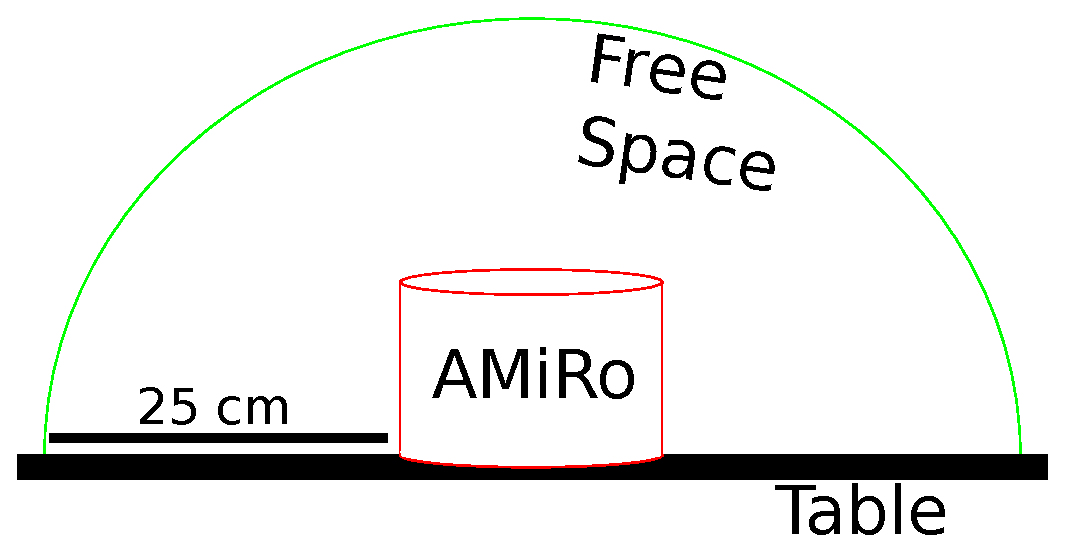
\includegraphics[scale=0.35]{Bilder/MeasGroundOffset.eps} \\
(a) Setup for air offsets & (b) Setup for ground offsets \\
\end{tabular}
\caption{Initialization setup for measuring the air offsets (a) and the ground offsets (b).}
\label{fig:proxinit}
\end{center}
\end{figure}

For the ground offset the \amiro\ has to be placed on the ground without any objects or edges around it (about \unit[25]{cm}) as shown in figure \ref{fig:proxinit}(b). Now {\it runIRConfig.sh} has to be executed. This will take several minutes. Afterwards in the project folder there should be a file named {\it irConfig.conf}, which contains the ground offsets of the actual surface the robot is standing on. Of course, the ground offsets depend on the ground, so this initialization has to be done for every ground, which shall be used.

For checking the offsets the following tools can be used: By executing {\it senseRingProximity} with the parameter {\it -p} the original values and the values for the obstacle and the edge model are printed. If the robot is on the ground without any object or edge in range, the obstacle values should be near zero, while the edge values should be near 10000. By executing {\it edgeMeasurement} (without any parameters) the edge distances for each sensor will be printed. The maximum distance is about \unit[6.5]{cm}.

\subsection{Capacity Touch Sensors}

\working

\subsection{Gyroscope}

\working

\subsection{Accelerometer}

\working

\subsection{Magnetometer}

\working

\subsection{Camera}

\working

\section{Actors}

The basic structure of the \amiro\ consisting of the modules \diwheel, \power\ and \light\ doesn't have much action. There are only driving actions and giving light signals.

\subsection{Motors}

The \diwheel\ controls the driving behavior of the \amiro. By giving CAN commands the driving velocity can be set and read. The motors cannot be commanded directly, but a forward velocity and an angle velocity can be given, which will be transformed in motor velocities by the \diwheel.

\medskip

\begin{tabular}{l|l}
{\bf CAN command} & {\bf Description} \\
\hline
{\tt void setTargetSpeed} & Sets the driving speed consisting of the forward \\
\quad {\tt int v} & velocity {\it v} and the angle velocity {\it w} \\
\quad {\tt int w} & \\
\hline
{\tt int getActualSpeed} & Reads the actual forward velocity {\it v} and the actual \\
\quad {\tt int v} & angle velocity {\it w}. If the values could be read, the return \\
\quad {\tt int w} & value will be zero. \\
\end{tabular}

\bigskip

There are still other CAN commands for driving like {\it setTargetPosition}, but these functions are deprecated! Please, only use the functions listed in the table.

\subsection{Lights}
\label{sec:lights}

The \light\ consists of eight RGB LEDs which are placed directly above the proximity sensors in the \proxring. The lights can only be set, but not read. The ID assignments for the LEDs are defined in figure \ref{fig:lightids}.

\begin{figure}[htb]
\begin{center}
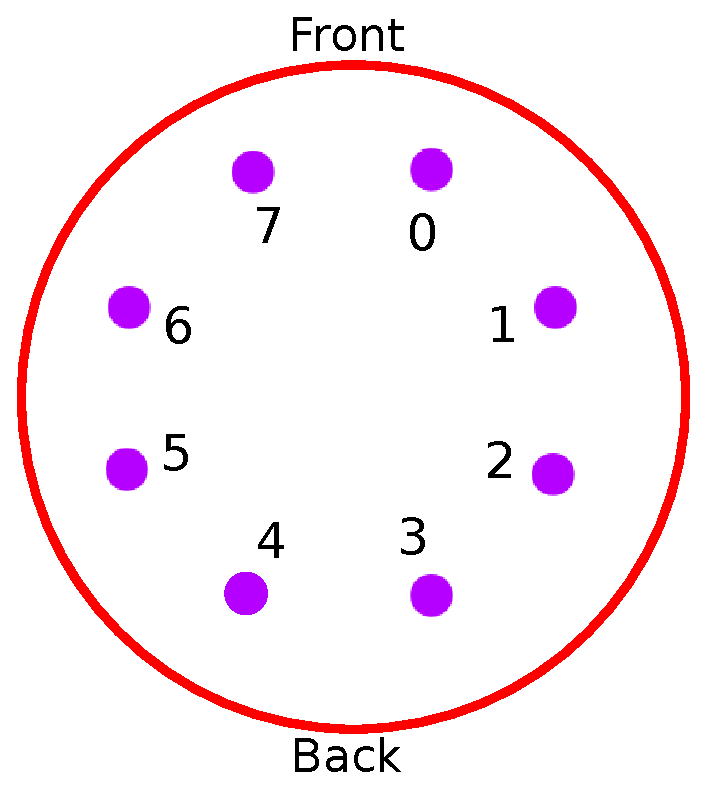
\includegraphics[scale=0.35]{Bilder/LightIDs.eps}
\caption{Top view of the \light\ with the ID assignments of the LEDs.}
\label{fig:lightids}
\end{center}
\end{figure}

There are two different possibilities to set the colors of the LEDs. The first one is setting the colors directly via CAN by the following functions:

\medskip

\begin{tabular}{l|l}
{\bf CAN command} & {\bf Description} \\
\hline
{\tt void setLightColor} & Sets the LED with the ID {\it index} on the given color. \\
\quad {\tt int index} & \\
\quad {\tt Color color} & \\
\hline
{\tt void setLightBrightness} & Sets the brightness of all LEDs. \\
\quad {\tt int brightness} & \\
\end{tabular}

\bigskip

The second way is to use the \setlightsnameI\ tool in \setlightspathI. It listens to an integer vector via RSB. Additionally to setting the colors, this tool can also blink the LEDs in different lighting types for given period times, so this tool is recommended, when the LEDs shall show special behaviors:

\medskip

\begin{tabular}{l|l}
{\bf Lighting Type} & {\bf Description} \\
\hline
{\tt SINGLE\_INIT}        & Sets the initial colors. \\
\hline
{\tt SINGLE\_SHINE}       & Sets the given colors and lets it just shine. \\
\hline
{\tt SINGLE\_BLINK}       & Sets the given colors and blinks with all LEDs turned on \\
                          & or off. \\
\hline
{\tt SINGLE\_WARNING}     & Sets the given colors and blinks with always the left or \\
                          & right half turned on or off. \\
\hline
{\tt SINGLE\_CROSSED}     & Sets the given colors and blinks with only 4 crossed LEDs \\
                          & at once turned on. \\
\hline
{\tt SINGLE\_CIRCLELEFT}  & Sets the given colors and lets circle two LEDs turned on \\
                          & to the left (counter clockwise). \\
\hline
{\tt SINGLE\_CIRCLERIGHT} & Sets the given colors and lets circle two LEDs turned on \\
                          & to the right (clockwise) \\
\hline
{\tt CHANGE\_INIT}        & Changes the colors without turning off the LEDs. The color \\
                          & set equals the initial colors. \\
\hline
{\tt CHANGE\_SHINE}       & Changes the given colors without turning off the LEDs. \\
\hline
{\tt CHANGE\_BLINK}       & Changes the given colors and blinks with all LEDs turnes on \\
                          & or off. \\
\end{tabular}

\bigskip

If the suffix {\tt SHINE} is used, then there can be given 1 color for all LEDs or 8 colors for each LED. While the chosen action the color of a single LED won't change. If the suffix {\tt CHANGE} is used, then there can be given many colors. In this case all LEDs will have the same color at the same time. The colors of every LED will change with each step of the chosen action.

Please use the {\it LightType} enumeration in the {\it LightModel.h} in {\it project/includes/actModels/}. There can be also find a more detailed documentation of the {\it LightType} in the file {\it startLightModel.txt}. As an example code the tool {\it sendLights} in {\it project/tools/examples/} shows, how to use the {\it LightModel.h} and how to generate and send the light command to the \setlightsnameI\ tool.



\newpage

\bibliographystyle{alpha}
\bibliography{ALiterature}
\appendix
\chapter{RSB Logger Output for Detailed Style}


\begin{figure}[htb]
\begin{center}
\includegraphics[scale=0.55]{Bilder/rsbloggerpics/rsb_br_simple_detailed.png}
\caption{Detailed style output of the scope {\it /rir\-prox/original} of the RSB logger of the simple Braitenberg demo.}
\label{fig:rsbloggersimpledetailed}
\end{center}
\end{figure}


\begin{figure}[htb]
\begin{center}
\includegraphics[scale=0.55]{Bilder/rsbloggerpics/rsb_br_standard_detailed-obstacleFront.png} \\
(a) \\
\quad\\
\includegraphics[scale=0.55]{Bilder/rsbloggerpics/rsb_br_standard_detailed-command.png} \\
(b)
\caption{Detailed style output of the scope {\it /rir\-prox/obstacle} in (a) and of the scope {\it /frontObject/command} in (b) of the RSB logger of the standard Braitenberg demo.}
\label{fig:rsbloggerstandarddetailed}
\end{center}
\end{figure}

\end{document}